% Font options: 10pm, 11pt, 12pt
% Align headings left instead of center: nocenter
\documentclass[xcolor=x11names,compress]{beamer}\usepackage[]{graphicx}\usepackage[]{color}
%% maxwidth is the original width if it is less than linewidth
%% otherwise use linewidth (to make sure the graphics do not exceed the margin)
\makeatletter
\def\maxwidth{ %
  \ifdim\Gin@nat@width>\linewidth
    \linewidth
  \else
    \Gin@nat@width
  \fi
}
\makeatother

\definecolor{fgcolor}{rgb}{0.345, 0.345, 0.345}
\newcommand{\hlnum}[1]{\textcolor[rgb]{0.686,0.059,0.569}{#1}}%
\newcommand{\hlstr}[1]{\textcolor[rgb]{0.192,0.494,0.8}{#1}}%
\newcommand{\hlcom}[1]{\textcolor[rgb]{0.678,0.584,0.686}{\textit{#1}}}%
\newcommand{\hlopt}[1]{\textcolor[rgb]{0,0,0}{#1}}%
\newcommand{\hlstd}[1]{\textcolor[rgb]{0.345,0.345,0.345}{#1}}%
\newcommand{\hlkwa}[1]{\textcolor[rgb]{0.161,0.373,0.58}{\textbf{#1}}}%
\newcommand{\hlkwb}[1]{\textcolor[rgb]{0.69,0.353,0.396}{#1}}%
\newcommand{\hlkwc}[1]{\textcolor[rgb]{0.333,0.667,0.333}{#1}}%
\newcommand{\hlkwd}[1]{\textcolor[rgb]{0.737,0.353,0.396}{\textbf{#1}}}%
\let\hlipl\hlkwb

\usepackage{framed}
\makeatletter
\newenvironment{kframe}{%
 \def\at@end@of@kframe{}%
 \ifinner\ifhmode%
  \def\at@end@of@kframe{\end{minipage}}%
  \begin{minipage}{\columnwidth}%
 \fi\fi%
 \def\FrameCommand##1{\hskip\@totalleftmargin \hskip-\fboxsep
 \colorbox{shadecolor}{##1}\hskip-\fboxsep
     % There is no \\@totalrightmargin, so:
     \hskip-\linewidth \hskip-\@totalleftmargin \hskip\columnwidth}%
 \MakeFramed {\advance\hsize-\width
   \@totalleftmargin\z@ \linewidth\hsize
   \@setminipage}}%
 {\par\unskip\endMakeFramed%
 \at@end@of@kframe}
\makeatother

\definecolor{shadecolor}{rgb}{.97, .97, .97}
\definecolor{messagecolor}{rgb}{0, 0, 0}
\definecolor{warningcolor}{rgb}{1, 0, 1}
\definecolor{errorcolor}{rgb}{1, 0, 0}
\newenvironment{knitrout}{}{} % an empty environment to be redefined in TeX

\usepackage{alltt}
%\documentclass[xcolor=x11names,compress,handout]{beamer}
\usepackage[]{graphicx}
\usepackage[]{color}
\usepackage{booktabs}
\usepackage{hyperref}
\usepackage{tikz}
\usepackage{multirow}
\usepackage{multicol}
\usepackage{dcolumn}
\usepackage{bigstrut}
\usepackage{amsmath} 
\usepackage{xcolor,colortbl}
\usepackage{amssymb}
%\newcommand{\done}{\cellcolor{teal}#1}

%% Beamer Layout %%%%%%%%%%%%%%%%%%%%%%%%%%%%%%%%%%
\useoutertheme[subsection=false,shadow]{miniframes}
\useinnertheme{default}
\usefonttheme{serif}
\usepackage{Arev}
\usepackage{pdfpages}

\setbeamerfont{title like}{shape=\scshape}
\setbeamerfont{frametitle}{shape=\scshape, size=\normalsize}

\definecolor{dkblue}{RGB}{0,0,102}

\setbeamercolor*{lower separation line head}{bg=dkblue} 
\setbeamercolor*{normal text}{fg=black,bg=white} 
\setbeamercolor*{alerted text}{fg=red} 
\setbeamercolor*{example text}{fg=black} 
\setbeamercolor*{structure}{fg=black} 
 
\setbeamercolor*{palette tertiary}{fg=black,bg=black!10} 
\setbeamercolor*{palette quaternary}{fg=black,bg=black!10} 

\renewcommand{\(}{\begin{columns}}
\renewcommand{\)}{\end{columns}}
\newcommand{\<}[1]{\begin{column}{#1}}
\renewcommand{\>}{\end{column}}

\setbeamertemplate{navigation symbols}{} 
\setbeamertemplate{footline}[frame number]
\setbeamertemplate{caption}{\raggedright\insertcaption\par}

\setbeamersize{text margin left=5pt,text margin right=5pt}

%%%%%%%%%%%%%%%%%%%%%%%%%%%%%%%%%%%%%%%%%%%%%%%%%%




\title{FLS 6441 - Methods III: Explanation and Causation}
\subtitle{Week 1 - Review}
\author{Jonathan Phillips}
\date{February 2019}
\IfFileExists{upquote.sty}{\usepackage{upquote}}{}
\begin{document}

\frame{\titlepage}

\section{Introduction}

\begin{frame}
\frametitle{Course Objectives}
\begin{enumerate}
\item temp
\end{enumerate}
\end{frame}

\section{Probability and Statistics in 10 minutes}

\begin{frame}
\frametitle{Data}
\begin{enumerate}
\item We work with variables, which VARY!
\end{enumerate}
\begin{kframe}
\begin{alltt}
\hlstd{data} \hlkwb{<-} \hlkwd{tibble}\hlstd{(}\hlkwc{Variable}\hlstd{=}\hlkwd{rnorm}\hlstd{(}\hlnum{10000}\hlstd{,}\hlnum{0}\hlstd{,}\hlnum{1}\hlstd{))}
\hlstd{data} \hlopt \hlkwd{slice}\hlstd{(}\hlnum{1}\hlopt{:}\hlnum{10}\hlstd{)} \hlopt \hlkwd{stargazer}\hlstd{()}
\end{alltt}
\end{kframe}
% Table created by stargazer v.5.2.2 by Marek Hlavac, Harvard University. E-mail: hlavac at fas.harvard.edu
% Date and time: Wed, Feb 27, 2019 - 8:53:54 PM
\begin{table}[!htbp] \centering 
  \caption{} 
  \label{} 
\begin{tabular}{@{\extracolsep{5pt}}lccccccc} 
\\[-1.8ex]\hline 
\hline \\[-1.8ex] 
Statistic & \multicolumn{1}{c}{N} & \multicolumn{1}{c}{Mean} & \multicolumn{1}{c}{St. Dev.} & \multicolumn{1}{c}{Min} & \multicolumn{1}{c}{Pctl(25)} & \multicolumn{1}{c}{Pctl(75)} & \multicolumn{1}{c}{Max} \\ 
\hline \\[-1.8ex] 
\hline \\[-1.8ex] 
\end{tabular} 
\end{table} 

\begin{knitrout}
\definecolor{shadecolor}{rgb}{0.969, 0.969, 0.969}\color{fgcolor}\begin{kframe}
\begin{alltt}
\hlstd{data} \hlopt \hlkwd{ggplot}\hlstd{()} \hlopt{+}
  \hlkwd{geom_line}\hlstd{(}\hlkwd{aes}\hlstd{(}\hlkwc{x}\hlstd{=Variable),} \hlkwc{stat}\hlstd{=}\hlstr{"density"}\hlstd{)} \hlopt{+}
  \hlkwd{theme_classic}\hlstd{()}
\end{alltt}
\end{kframe}
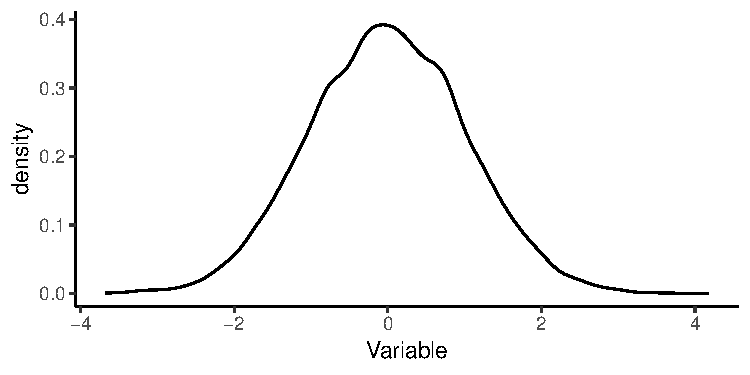
\includegraphics[width=\maxwidth]{figure/var2-1} 

\end{knitrout}
\end{frame}

\section{What does Regression do?}

\begin{frame}
\frametitle{Probability}
\begin{enumerate}
\item temp
\end{enumerate}
\end{frame}

\section{Guide to Designing Regressions}

\begin{frame}
\frametitle{Regression Guide}
\begin{enumerate}
\item \textbf{Choose variables and measures:} To test a specific hypothesis
\item \textbf{Choose a Model/Link Function:} Should match the data type of your outcome variable
\item \textbf{Choose Covariates:} To match your strategy of inference
\item \textbf{Choose Fixed Effects:} To focus on a specific level of variation
\item \textbf{Choose Standard Error Structure:} To match known dependencies/clustering in the data
\item \textbf{Interpret the coefficients:} Depending on the type/scale of the explanatory variable
\end{enumerate}
\end{frame}

\begin{frame}
\frametitle{Regression Models}
The Regression Model reflects the data type of the outcome variable:
\begin{itemize}
\item Continuous -> Ordinary Least Squares  
\begin{knitrout}
\definecolor{shadecolor}{rgb}{0.969, 0.969, 0.969}\color{fgcolor}\begin{kframe}
\begin{alltt}
\hlstd{d} \hlopt \hlkwd{zelig}\hlstd{(Y} \hlopt{~} \hlstd{X,}\hlkwc{data}\hlstd{=.,}\hlkwc{model}\hlstd{=}\hlstr{"ls"}\hlstd{)}
\end{alltt}
\end{kframe}
\end{knitrout}
\item Binary -> Logit  
\begin{knitrout}
\definecolor{shadecolor}{rgb}{0.969, 0.969, 0.969}\color{fgcolor}\begin{kframe}
\begin{alltt}
\hlstd{d} \hlopt \hlkwd{zelig}\hlstd{(Y} \hlopt{~} \hlstd{X,}\hlkwc{data}\hlstd{=.,}\hlkwc{model}\hlstd{=}\hlstr{"logit"}\hlstd{)}
\end{alltt}
\end{kframe}
\end{knitrout}
\item Unordered categories -> Multinomial logit  
\begin{knitrout}
\definecolor{shadecolor}{rgb}{0.969, 0.969, 0.969}\color{fgcolor}\begin{kframe}
\begin{alltt}
\hlstd{d} \hlopt \hlkwd{zelig}\hlstd{(Y} \hlopt{~} \hlstd{X,}\hlkwc{data}\hlstd{=.,}\hlkwc{model}\hlstd{=}\hlstr{"mlogit"}\hlstd{)}
\end{alltt}
\end{kframe}
\end{knitrout}
\item Ordered categories -> Ordered logit  
\begin{knitrout}
\definecolor{shadecolor}{rgb}{0.969, 0.969, 0.969}\color{fgcolor}\begin{kframe}
\begin{alltt}
\hlstd{d} \hlopt \hlkwd{zelig}\hlstd{(Y} \hlopt{~} \hlstd{X,}\hlkwc{data}\hlstd{=.,}\hlkwc{model}\hlstd{=}\hlstr{"ologit"}\hlstd{)}
\end{alltt}
\end{kframe}
\end{knitrout}
\item Count -> Poisson  
\begin{knitrout}
\definecolor{shadecolor}{rgb}{0.969, 0.969, 0.969}\color{fgcolor}\begin{kframe}
\begin{alltt}
\hlstd{d} \hlopt \hlkwd{zelig}\hlstd{(Y} \hlopt{~} \hlstd{X,}\hlkwc{data}\hlstd{=.,}\hlkwc{model}\hlstd{=}\hlstr{"poisson"}\hlstd{)}
\end{alltt}
\end{kframe}
\end{knitrout}
\end{itemize}
\end{itemize}
\end{frame}

\begin{frame}
\frametitle{Interpreting Regression Results}
\begin{itemize}
\item Difficult! It depends on the scale of the explanatory variable, scale of the outcome, the regression model we used, and the presence of any interaction
\item Basic OLS:
\begin{itemize}
\item 1 [unit of explanatory variable] change in the explanatory variable is associated with a $\beta$ [unit of outcome variable] change in the outcome
\end{itemize}
\end{itemize}
\end{frame}

\begin{frame}
\frametitle{Predictions from Regressions}
\begin{itemize}
\item temp
\end{itemize}
\end{frame}

%PVs for OLS, for logit, FDs
%PVs vs. EVs

\section{What does Regression NOT do?}

% Measurement Error
% Omitted Variable Bias
% Reverse Causation/Endogeneity
% Self-Selection Bias
% Data Selection Bias

\end{document}


%setwd('C:\\Users\\Jonny\\Google Drive\\Academic\\USP\\Class\\Week 1 - Intro\\Lecture Slides')
%knitr::knit("Slides_Wk1_intro_5.Rnw")
